\chapter[Softwarové Architektury]{B4M36SWA \\[1ex]\Large{Softwarové architektury, jejich parametry a kvalitativní metriky. Architektonické vzory, styly a standardy}}

Advantages
\begin{itemize}
    \item Productivity - coordinate work, implement features, guide discussions on potential issues
    \item Evolution - makes changes easier to accomplish or defects easier to find
    \item Quality - Enhance quality by considering the needs and perspectives of stakeholders
    \item Documentation - transferable, reusable abstraction
\end{itemize}

SWA is available in every single aspect in the software development lifecycle

\begin{itemize}
    \item Requirement - Requirements analysis
    \item Design - Domain-specific software architectures - best solutions and best practices from past projects; Reuse applicable parts
    \item Implementation - All of the structural elements found in the architecture are implemented in the source code
    \item Testing - transferable, reusable abstraction
\end{itemize}



\begin{itemize}
    \item \textbf{logical view} - functionality - class diagram and state diagram
    \item \textbf{process view} - Non-functional requirements - activity diagram and the sequence diagram
    \item \textbf{Development view} - implementation - hierarchical software structure, no standard diagram
    \item \textbf{Physical view} - physical components - deployment diagram
\end{itemize}

\begin{figure}[ht!]
\centering
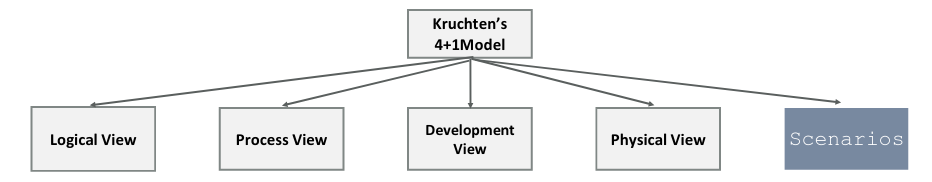
\includegraphics[width=\textwidth]{oborove/SWA/img/krutchen.png}
\end{figure}


\section{Quality attributes}
\begin{figure}[ht!]
\centering
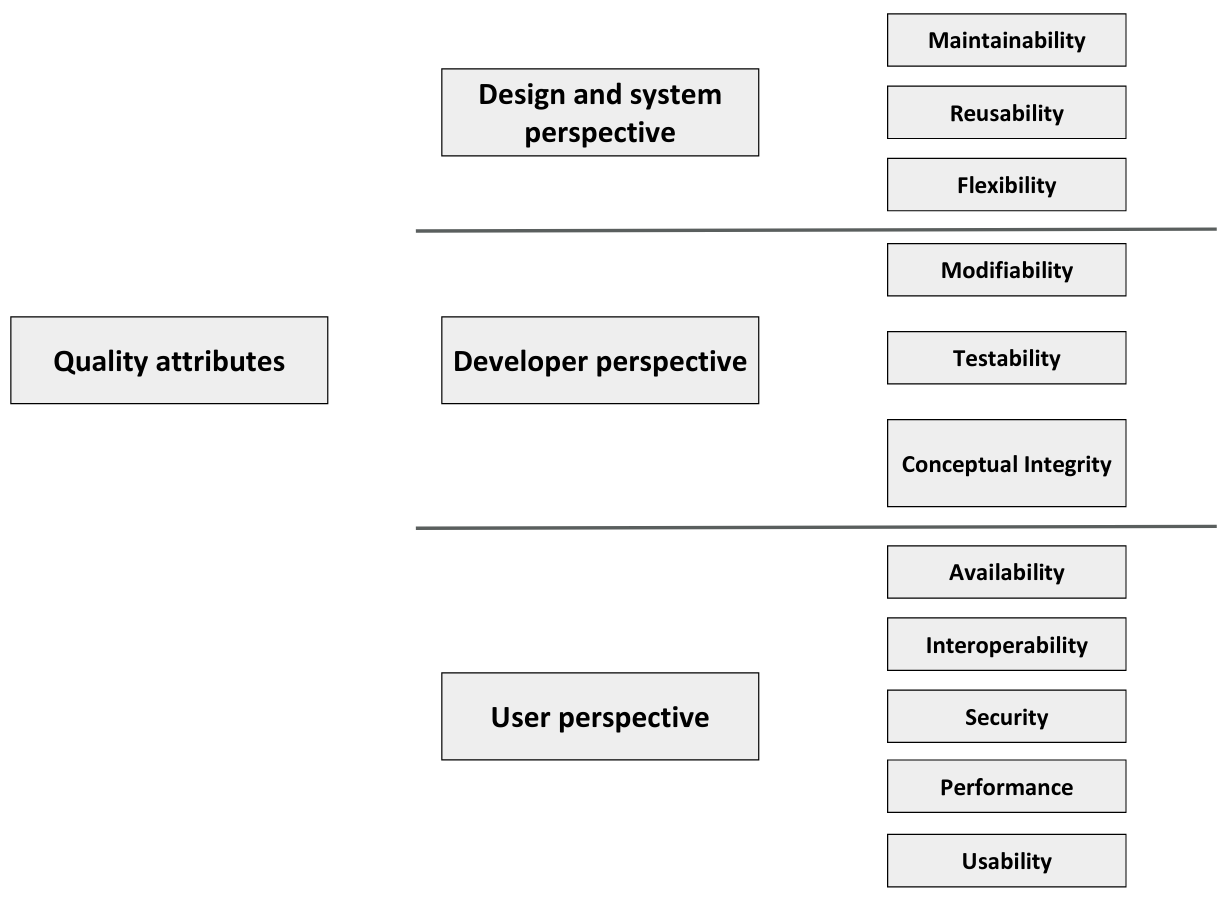
\includegraphics[width=0.75\textwidth]{oborove/SWA/img/quality.png}
\end{figure}


\begin{itemize}
    \item \textbf{Maintainability} - ease at which your system is capable of undergoing changes.
    \item \textbf{Reusability} - The extent in which functions or parts of your system can be used in another
    \item \textbf{Flexibility} - How well a system can adapt to requirements change
    \item \textbf{Modifiability} - ability of a system to cope with changes
    \item \textbf{Testability} - How easy it is to demonstrate errors through executable tests.
    \item \textbf{Conceptual Integrity} - consistency across the entire system
    \item \textbf{Interoperability} - ability of your system to understand communications and share data with external systems
    \item \textbf{Security} - ability to protect sensitive data from unauthorized and unauthenticated use
    \item \textbf{Availability} - amount of time the system is operational over a set period of time
    \item \textbf{Performance} - throughput and latency
    \item \textbf{Usability} - ease at which the system’s functions can be learned and used by the end users
\end{itemize}

ISO/IEC 25010:2011 Quality Model

\begin{figure}[ht!]
\centering
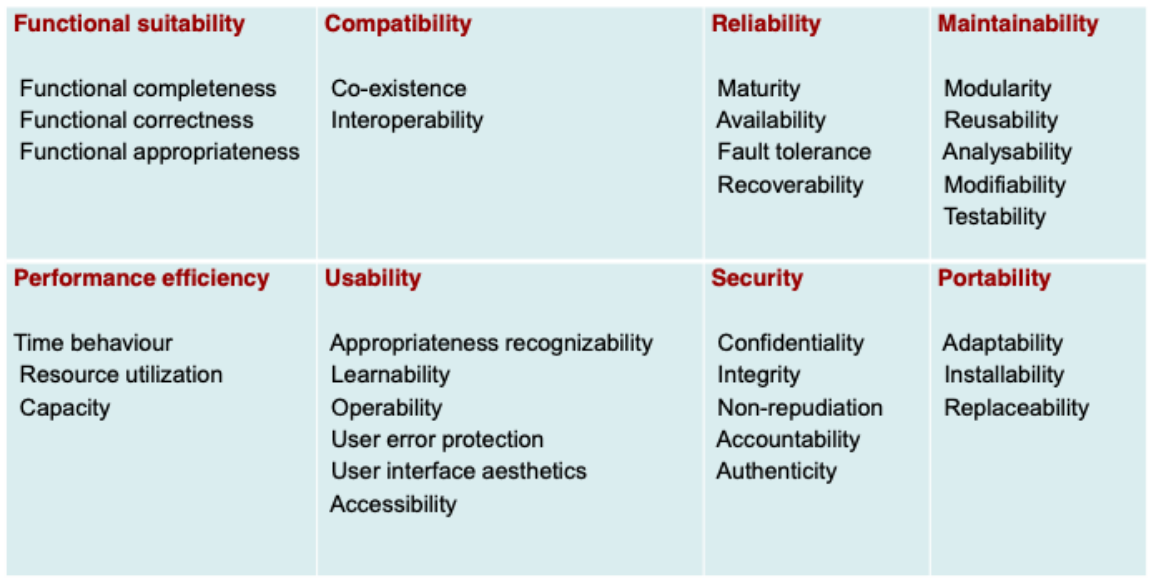
\includegraphics[width=\textwidth]{oborove/SWA/img/ieee_quality.png}
\end{figure}

\textbf{Evaluating Quality Attributes}
\begin{itemize}
    \item \textbf{Scenario-based evaluation}
    \item \textbf{Simulation} - prototyping
    \item \textbf{Mathematical modeling} - deadlock checks
    \item \textbf{Experience-based assessment} - subjective
\end{itemize}

\pagebreak
\textbf{Scenarios}
\begin{figure}[ht!]
\centering
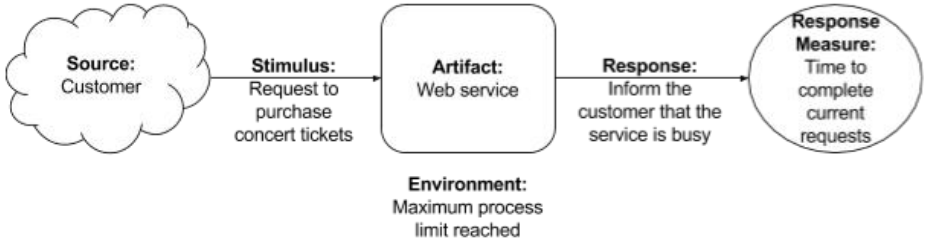
\includegraphics[width=\textwidth]{oborove/SWA/img/scenarios.png}
\end{figure}

Scenarios involving incorrect input, heavy system loads, or potential security breaches should be prioritized highly

\textbf{Architecture Trade-off Analysis Method}
\begin{figure}[ht!]
\centering
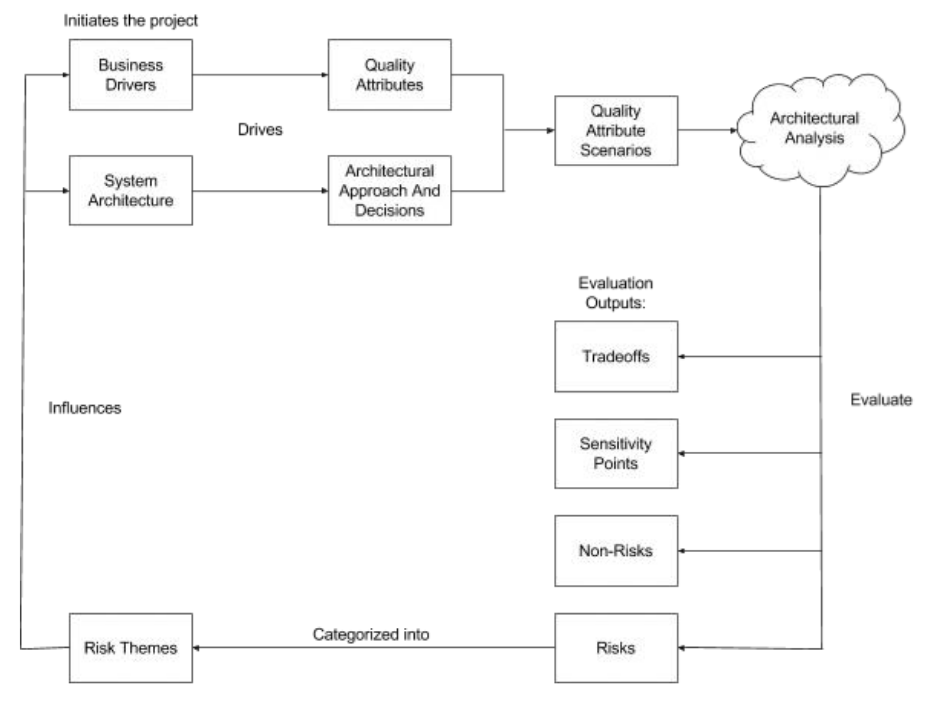
\includegraphics[width=\textwidth]{oborove/SWA/img/ATAM.png}
\end{figure}

\pagebreak
\begin{figure}[ht!]
\centering
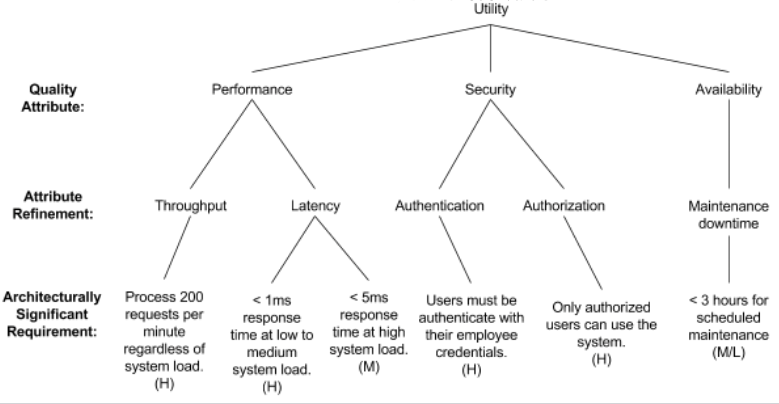
\includegraphics[width=\textwidth]{oborove/SWA/img/tree.png}
\end{figure}

\section{Software Architecture}

\textbf{Some principles:}

\begin{itemize}
    \item Separation of concerns
    \item Single responsibility principle
    \item Keep it simple, stupid (KISS)
    \item Don’t repeat yourself (DRY)
    \item Don’t talk to strangers (Demeter’s law)
    \item You aren’t gonna need it (YAGNI)
    \item Inversion of Control (IoC)
    \item Dependency injection (DI)
    \item Data Access Object (DAO)
    \item Model View Controller (MVC)
    \item Hollywood principle (Don't Call Us, We'll Call You)
    \item High cohesion, loose coupling
\end{itemize}

\textbf{Architectural styles}

\textbf{Communication}
Service-Oriented Architecture - Microservices

Event-driven Architecture - Events are emitted (published), subscribers are notified

Message Bus - Central message queue handles message distribution

\textbf{Deployment}

Client/Server - Server – possible single point of failures

N-tier - Independent tiers providing functionality

\textbf{Structure}

Component-based - System decomposed into logical or functional components

Object-oriented - Objects consist of both behaviour and data

Layered - Layers of related functionality

Hexagonal architecture - aka ports and adapters

\textbf{Data}

Blackboard - Knowledge sources operate over a common global memory – the blackboard
Pipes and Filters - Data flow through pipes between filters; Filters are independent, self-contained processing components

\textbf{Other}

Domain-driven Design - Business components represent domain entities

Aspect-oriented Programming - Hook into important runtime events – instantiation, method invocation etc. – and run additional code

\textbf{Design patterns}

\textbf{Creational Patterns}
\begin{itemize}
    \item Abstract Factory Interface for creating families of related objects
    \item Builder Instance construction process in a separate object
    \item Factory Method Subclasses decide which class to instantiate
    \item Prototype Build instances based on a prototype
    \item Singleton Only one instance of the class
\end{itemize}

\textbf{Structural Patterns}
\begin{itemize}
    \item Adapter Convert the interface of one class to a different interface using an adapter (e.g., for legacy classes)
    \item Bridge Decouple abstraction from implementation
    \item Composite Build a tree-like structure of objects
    \item Decorator Add or alter behaviour of another object by wrapping it in a class with the same interface (e.g., Java I/O streams)
    \item Facade Provide a unified interface to a set of interfaces
    \item Flyweight Use sharing to support a large number of fine-grained objects
    \item Proxy Provide a placeholder for another object to control access to it (e.g. Spring bean proxies)
\end{itemize}

\textbf{Behavioral Patterns}
\begin{itemize}
    \item Chain of Responsibility Multiple objects in a chain can handle a request (e.g., request filters)
    \item Command Encapsulate a request in an object (e.g., undo functionality)
    \item Interpreter Interpreter for a language and its grammar
    \item Iterator Provide a way to access elements of an aggregate object (e.g., Java collections)
    \item Mediator An object that encapsulates how a set of objects interact
    \item Memento Capture an object’s state so that it can be restored to this state later
    \item Observer Decoupled notification of changes of object’s state
    \item State Allows object’s behaviour to change based on its internal state
    \item Strategy A family of algorithms which can be interchanged independently of the client
    \item Template method Define a skeleton of an algorithm and let subclasses fill in the details
    \item Visitor Represent an operation to be performed on the elements of an object structure
\end{itemize}


\textbf{Enterprise Design Patterns}

Data Transfer Object (DTO) - Object that carries data between processes in order to reduce the number of calls

Lazy Load - Object does not contain all of its data initially, but knows how to load it

Model View Controller (MVC) - Splits user interface interaction into three distinct roles

\begin{figure}[ht!]
\centering
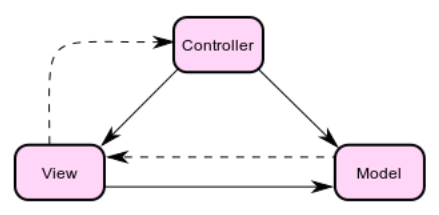
\includegraphics[width=.6\textwidth]{oborove/SWA/img/mvc.png}
\end{figure}

Unit Of Work - Maintains objects affected by a business transaction and coordinates the writing out of changes and the resolution of concurrency problems

\section{Rest services}
Uniform Resource Identifier (URI) is a string of characters used to identify a resource 

The Hypertext Transfer Protocol (HTTP) is an application protocol

Representational State Transfer (REST) is an architectural style for distributed hypermedia systems

REST is an architectural style, not standard!


HTTP REQUEST LINE - Request: <TYPE> <URI> <VER> \newline Status: <VER> <STATUS> <MSG>

\textbf{HTTP Headers}
\begin{figure}[ht!]
\centering
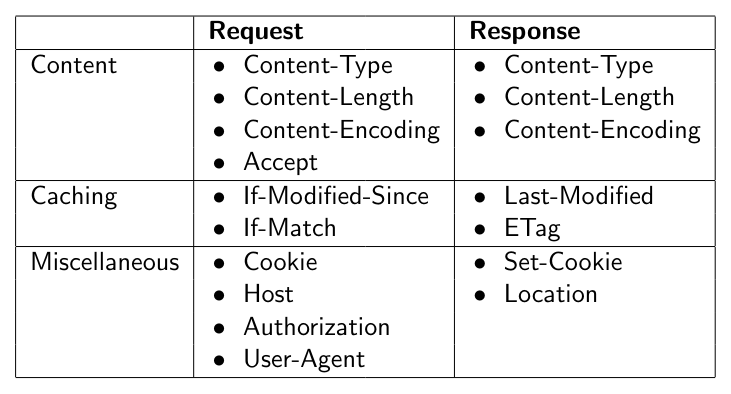
\includegraphics[width=.75\textwidth]{oborove/SWA/img/http_headers.png}
\end{figure}

\textbf{GET} - Used to retrieve resource at request URI

\textbf{POST} - Requests server to create new resource from the specified body

\textbf{PUT} - Requests server to store the specified entity under the request URI

\textbf{DELETE} - Used to ask server to delete resource at the request URI


\textbf{HTTP CODES}

\textbf{1XX} - Rarely used

\textbf{2XX} - Success

\textbf{3XX} - Redirection

\textbf{4XX} - Client error

\textbf{5XX} - Server error

\textbf{Rest principles}

\begin{itemize}
    \item Client-server
    \item Uniform interface - Resource-based Manipulation of resource through representation Self-descriptive messages
    \item Stateless interactions
    \item Cacheable
    \item Layered system
    \item Code on demand (optional) 
\end{itemize}

Resources should have name as nouns, not as verbs or actions, plural if possible, URI should follow a predictable (i.e., consistent usage) and hierarchical structure
\pagebreak
\section{Microservices}
Monolith - Code base grows and becomes more complex
\begin{figure}[ht!]
\centering
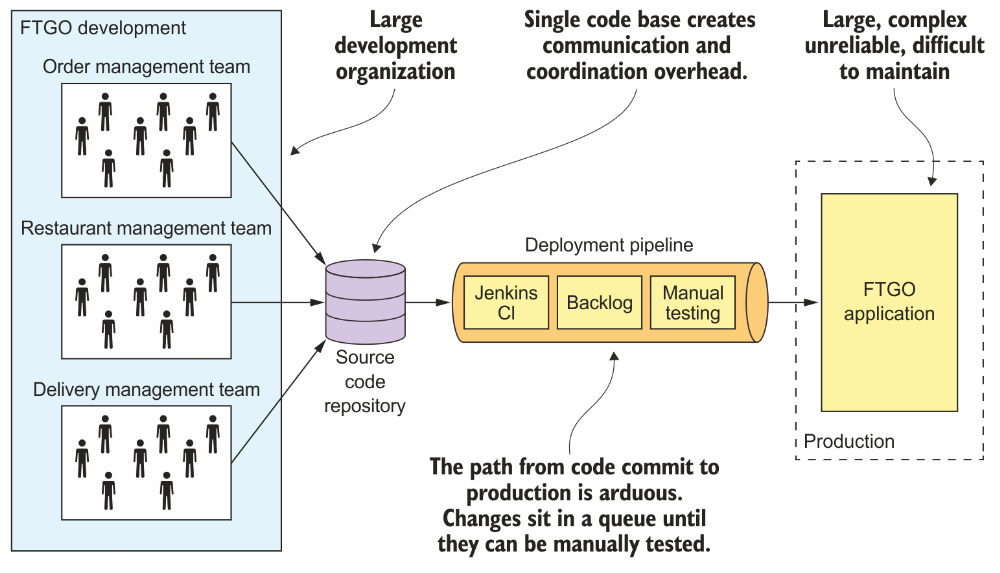
\includegraphics[width=.75\textwidth]{oborove/SWA/img/monolith.png}
\end{figure}

Microservices - small, independent, scalable
\begin{figure}[ht!]
\centering
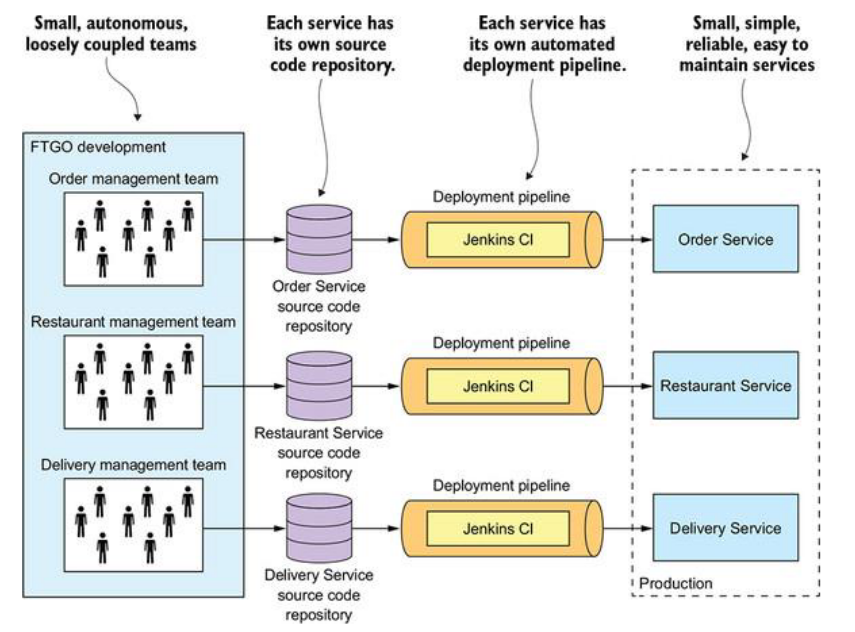
\includegraphics[width=.75\textwidth]{oborove/SWA/img/microservice.png}
\end{figure}

Each of the many microservices might failDesign every service assuming that at some point, everything it depends on might disappear – must  fail “gracefully”

\textbf{TECHNICAL ANTIPATTERNS}

\begin{itemize}
    \item API Versioning – APIs are not semantically versioned, also known as “Static contract pitfall”
    \item Inappropriate Service Intimacy – service keeps asking other service for data
    \item Megaservice – also known as “Monolith”
    \item Cyclic Dependency – a cyclic chain between services
    \item ESB Usage – communication via Enterprise Service Bus which includes additional complexity and is not lightweight
    \item No API-Gateway – services connect to each other directly
    \item Shared Libraries – couples services together, problems with modification of such library, also know as “I was taough to share”
    \item Shared Persistence – couples services together, reduces service/team independence
    \item Wrong Cuts – wrong separation of concerns, increased data-splitting complexity
\end{itemize}

\textbf{ORGANIZATIONAL ANTIPATTERNS}

\begin{itemize}
    \item Legacy organization
    \item Non-homogenous Adoption - partial migration to microservices
    \item Common Ownership – one team owns all the microservices
    \item Microservice Greedy – microservice is created for each feature
    \item Lack of Microservice Skeleton – each team develops microservices from scratch without a benefit of shared skeleton
    \item No DevOps tools – manual testing and manual deployment because the company does not employ CI/CD
    \item Too Many Technologies – no common policy for service development, also known as “Lust” or “Glutony”
\end{itemize}

\textbf{THE ADOPTION ANTIPATTERNS}
\begin{itemize}
    \item Microservices are a magic pixie dust - believing that a sprinkle of microservices will solve all of your development problems
    \item Microservices as the goal - making the adoption of microservices the goal and measuring success in terms of the number of services written
    \item Scattershot adoption - multiple application development teams attempt to adopt the microservice architecture without any coordination
    \item Trying to fly before you can walk - attempting to adopt the microservice architecture (an advanced technique) without (or not committing to) practicing basic software development techniques, such as clean code, good design, and automated testing
    \item Focusing on Technology - focusing on technology aspects of microservices, most commonly the deployment infrastructure, and neglecting key issues, such as service decomposition
    \item More the merrier - intentionally creating a very fine-grained microservice architecture
    \item Red Flag Law - retaining the same development process and organization structure that were used when developing monolithic applications.
\end{itemize}

Ideally, each service should have only a small set of responsibilities - Single Responsibility Principle on service design level

\textbf{TWELWE-FACTOR APPLICATIONS}

\begin{enumerate}
    \item Codebase - One codebase tracked in revision control, many deploys
    \item Dependencies - Explicitly declare and isolate dependencies
    \item Config - Store config in the environment
    \item Backing services - Treat backing services as attached resources
    \item Build, release, run - Strictly separate build and run stages
    \item Processes - Execute the app as one or more stateless processes
    \item Port binding - Export services via port binding
    \item Concurrency - Scale out via the process model
    \item Disposability - Maximize robustness with fast startup and graceful shutdown
    \item Dev/prod parity - Keep development, staging, and production as similar as possible
    \item Logs - Treat logs as event streams
    \item Admin processes Run admin/management tasks as one-off processes
\end{enumerate}

\textbf{REACTIVE MANIFESTO}

Responsive - responds in a timely manner if possible

Resilient - responsive in the face of failure

Elastic - stays responsive under varying workload

Message Driven - rely on asynchronous message-passing

\textbf{CONWAY’S LAW}

Organizations which design systems are constrained to produce designs which are copies of the communication structures of these organizations to the extent that an organization is not completely flexible in its communication structure, that organization will stamp out an image of itself in every design it produces.

\section{MULTI-CONTAINER APPLICATIONS}
Systems have four general areas that scalability can apply to:
\begin{itemize}
    \item Disk I/O
    \item Memory
    \item Network I/O
    \item CPU
\end{itemize}


\textbf{X-axis}
\begin{figure}[ht!]
\centering
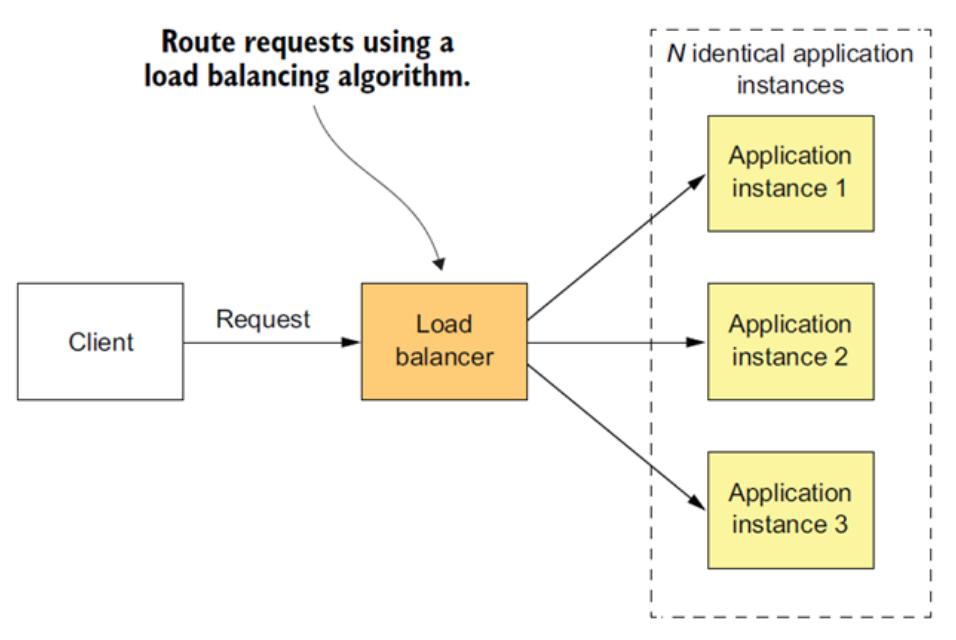
\includegraphics[width=0.8\textwidth]{oborove/SWA/img/x_axis.png}
\end{figure}

\pagebreak
\textbf{Y-axis}
\begin{figure}[ht!]
\centering
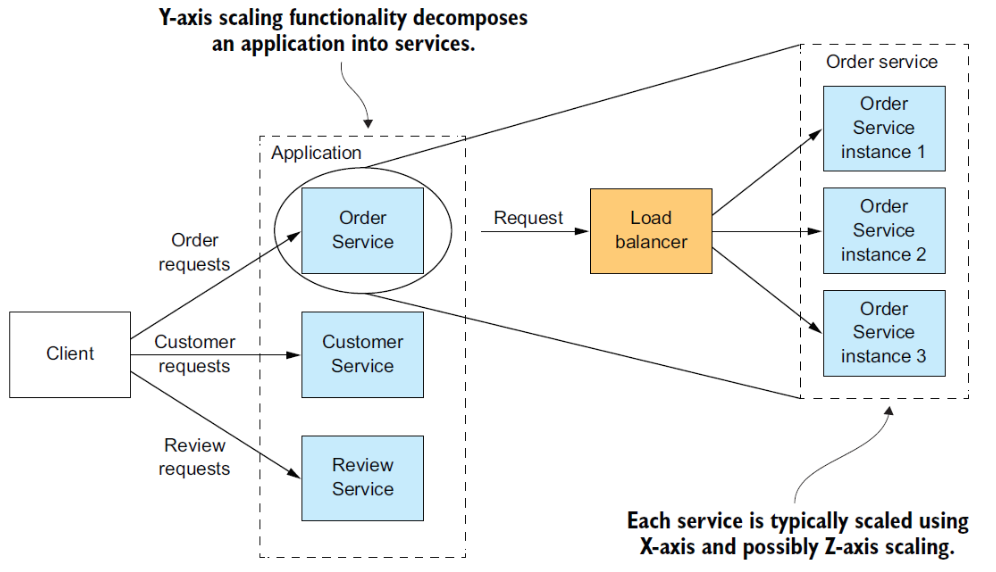
\includegraphics[width=\textwidth]{oborove/SWA/img/y_axis.png}
\end{figure}


\textbf{Z-axis}
\begin{figure}[ht!]
\centering
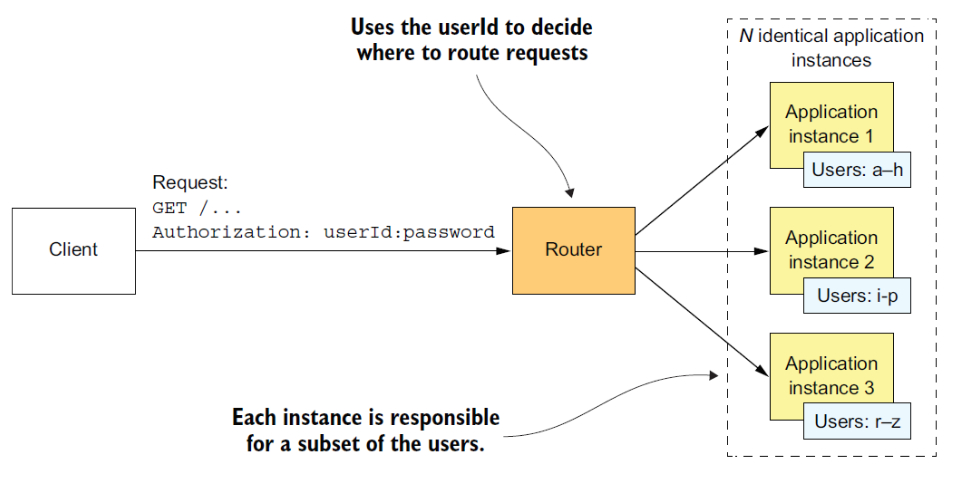
\includegraphics[width=\textwidth]{oborove/SWA/img/z_axis.png}
\end{figure}
\pagebreak

\textbf{ORCHESTRATION VS CHOREOGRAPHY} - Orchestration entails actively controlling all elements and interactions like a conductor directs the musicians of an orchestra, while choreography entails establishing a pattern or routine that microservices follow as the music plays, without requiring supervision and instructions
\begin{figure}[ht!]
\centering
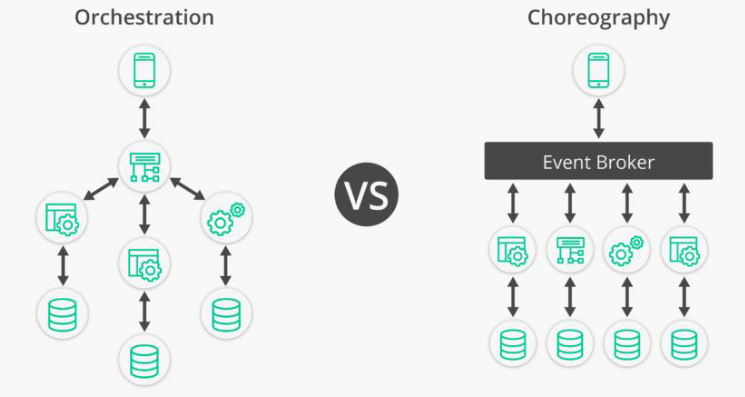
\includegraphics[width=\textwidth]{oborove/SWA/img/orch-vs-chor.png}
\end{figure}
\pagebreak

\textbf{SERVICE MESH} - Network of microservices that make up such applications and the interactions between them

\section{IoT}

Challenges:
\begin{itemize}
    \item Security - Low prices => updates might be impossible; lightweight security algo - low energy consumption... => IoT devices can serve as a weakpoint to get to whole network
    \item Privacy - Various personal data can be collectedLegislative issues being discussed in parallel with technology development => Opportunities to misuse of personal data are increasing; Low user's insight into data privacy mechanism
    \item Interoperability - Various protocols used –IPv6, Bluetooth, Intentional "vendor lockout" possible
    \item Reliability of service - Dependency of user to the network service growsdemands for service; availability continously grow => Need for an architecture supporting stabile operation of an IoT system
\end{itemize}


\textbf{One device / subsystem}

\textbf{Sense-Compute-Control}
\begin{figure}[ht!]
\centering
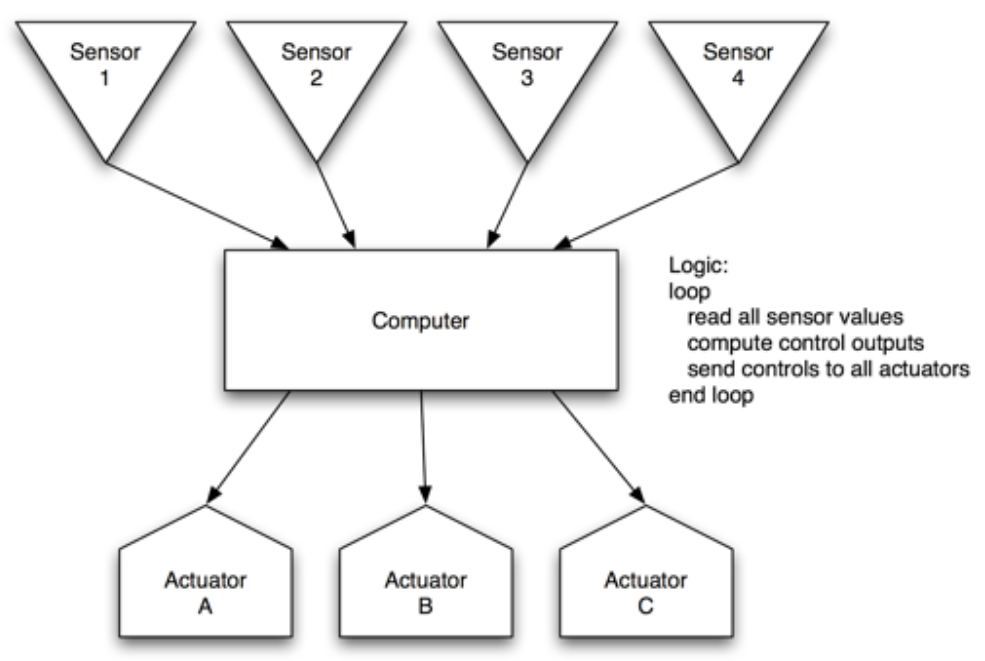
\includegraphics[width=.7\textwidth]{oborove/SWA/img/SCC.png}
\end{figure}
\pagebreak

\textbf{MAPE-K structure (Monitor-Analyze-Plan-Execute over a shared Knowledge)}
\begin{figure}[ht!]
\centering
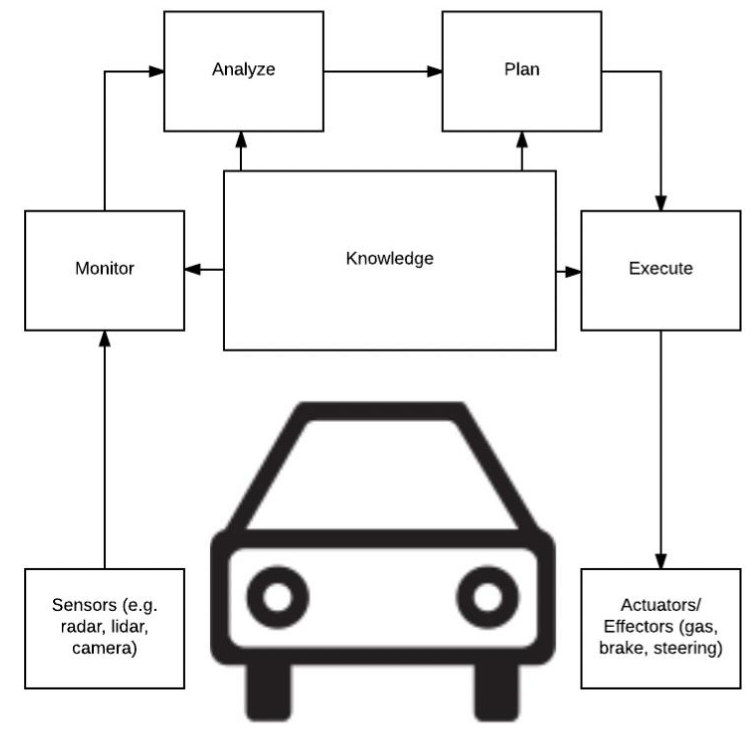
\includegraphics[width=.6\textwidth]{oborove/SWA/img/mapek.png}
\end{figure}

\textbf{Monitor:} The component or collection of components that interfaces with sensors, turning raw signals into meaningful information for the software.

\textbf{Analyze:} The software must next analyze this data. Data could be integrated from several sensors, so analysis might be quite sophisticated.

\textbf{Plan:} Next, planning needs to be done. More advanced planning needs will require more knowledge. This knowledge is in the form of a model of the system.

\textbf{Execute:}  The final step is to execute. Analysis and planning should make execution relatively simple. They will simply turn desired actuator positions into signals to communicate to those actuators

\textbf{Integrated system}\\
Gateway-centric architecture\\
Distributed IoT\\
Connected Intranets of Things\\
Collaborative IoT architecture\\
Wireless sensor network (WSN)